\section{Model}
\label{sec:model}

The basic element of our model is a \tg, which represents a graph that
evolves over time.  Our representation is based on a continuous time
domain.  This is in contrast to representing a graph as a sequence of
discrete states. We will discuss this distinction in detail in
Section~\ref{sec:model:others}.  We define the structure of an
evolving graph in Section~\ref{sec:model:structure}.  We then show the
relationship with other models in Section~\ref{sec:model:others}.
Finally, in Section~\ref{sec:model:algebra} we define the algebraic
operations on our model.

\subsection{Evolving Graphs}
\label{sec:model:structure}

First we describe how time is represented in our model.  Following the
SQL:2011 standard~\cite{DBLP:journals/sigmod/KulkarniM12}, we adopt
the {\em closed-open} period model, where a period represents all
times starting from and including the start time, continuing to but
excluding the end time.

\begin{definition}[Time period]
A {\em time period} \\$p = [start, end)$ is an interval on the
  continuous time domain $T$, subject to the constraint $start < end$.
\label{def:period} 
\end{definition}

\begin{definition}[TGraph]
An {\em evolving graph} $TG$ is a pair $(V;E)$, where $V$ is a finite
set of nodes with schema $(\underline{vid}, a_1, \ldots, a_n,
\underline{p})$, and $E$ is a finite set of edges connecting pairs of
nodes from $V$, with schema $(\underline{vid_1}, \underline{vid_2},
b_1, \ldots, b_m, \underline{p})$, and $p$ is a {\em maximally
  coalesced} time period.  Formally stated, the relationship between
$V$ and $E$ is through a constraint on $E$: $\forall e(vid_1, vid_2,
p_i) \in E, \exists v1(vid_1, p_j)$ and $v2(vid_2, p_k)$ and
$p_i.contains(p_j)$ and $p_i.contains(p_k)$.
\label{def:tg}
\end{definition}

\begin{figure}
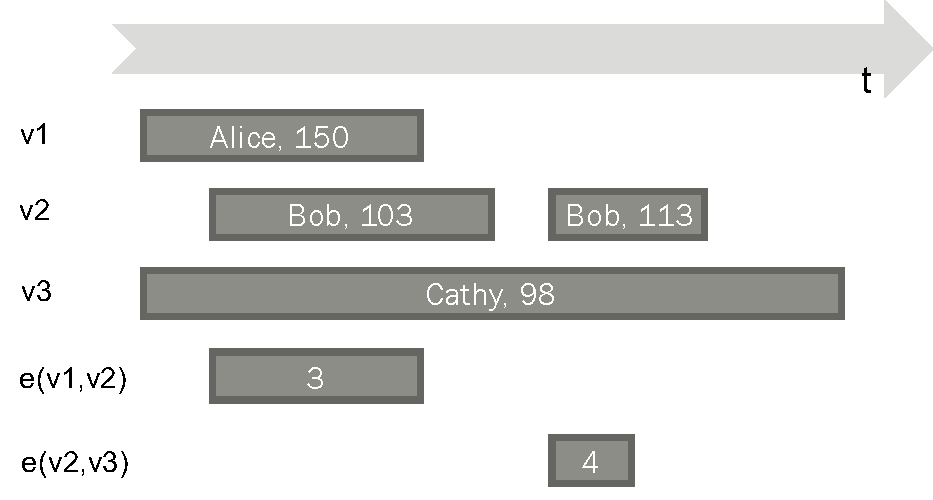
\includegraphics[width=3in]{figs/T1.pdf}
\caption{\tg \insql{T1} example.}
\label{fig:tg}
\end{figure}

An example of a \tg is given in Figure~\ref{fig:tg}, with vertex
schema name:string and salary:int and edge schema count:int.

The time periods of all graph entities, i.e. vertices and edges, are
maximally coalesced.  That means that all the tuples in $V$ and $E$
are distinct in all attributes, including the time periods, and that
time periods do not overlap for any individual entity and are maximal.
The above evolving graph definition~\ref{def:tg} can be expressed in
temporal SQL as follows (without attributes):

\begin{small}
\begin{verbatim}
CREATE TABLE V (
  vid LONG,
  estart DATE,
  eend DATE,
  PERIOD for eperiod (estart, eend),
  PRIMARY KEY (vid, eperiod WITHOUT OVERLAPS)
);
CREATE TABLE E (
  vid1 LONG,
  vid2 LONG,
  estart DATE,
  eend DATE,
  PERIOD for eperiod (estart, eend),
  PRIMARY KEY (vid1, vid2, eperiod WITHOUT OVERLAPS),
  FOREIGN KEY (vid1, PERIOD eperiod) 
           REFERENCES V(vid, PERIOD eperiod),
  FOREIGN KEY (vid2, PERIOD eperiod) 
           REFERENCES V(vid, PERIOD eperiod)
)
\end{verbatim}
\end{small}

\vera{placeholder for schema on load explanation}

\subsection{Other Models}
\label{sec:model:others}

There are two common ways to represent entities in time: continuous
and discrete.  We use a continous representation which is more general.

Much of the work on evolving graphs is on snapshot retrieval and
snapshot analytics in a discrete time domain.  In this case an
evolving graph is considered to be a sequence of graph snapshots
corresponding to time instances in the time domain $T$
(\cite{Khurana2013,DBLP:journals/tos/MiaoHLWYZPCC15,Ren2011}).  Such a
model has several limitations:

\begin{itemize}[noitemsep,topsep=0pt]
\item It requires a discrete time domain.  The state of the graph can
  be undefined at some time $t_i$ unless a snapshot is associated with
  each possible value of $T$ in the discrete range $[t_{start}, now)$.
\item It is not compact.  Every change to an entity (vertex or edge)
  requires a new snapshot.  For large graphs, consecutive snapshots
  have degree of similarity approaching 1 (on the scale of 0 of no
  similarity and 1 full similarity).
\end{itemize}

\begin{figure}[h]
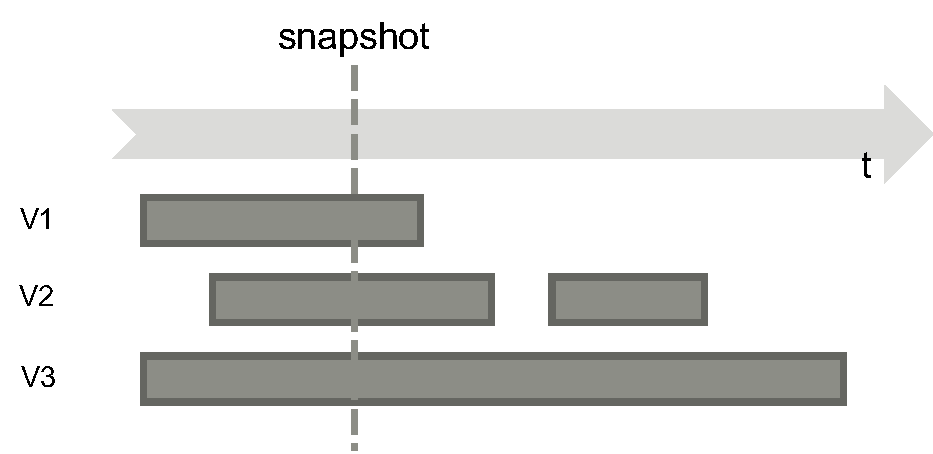
\includegraphics[width=3in]{figs/getsnap.pdf}
\caption{A graph snapshot over interval model TG is a time slice at time t.}
\label{fig:getsnap}
\end{figure}

Snapshot retrieval, however, is a useful operation for many types of
analysis and thus should be supported.  In our model a snapshot at any
time $t$ is state at time $t$ and can be retrieved simply by selection
on $p$ (Figure~\ref{fig:getsnap}). In SQL (similarly for E):

\begin{small}
\begin{verbatim}
SELECT *
FROM V
WHERE eperiod CONTAINS DATE ':date';
\end{verbatim}
\end{small}

Observe that many discrete dates can lead to equivalent snapshots if
no changes to the graph occurred in the intervening time.  It may be
desirable to instead retrieve a sequence of deduplicated snapshots
with respect to a subset of graph attributes.  We discuss how our
model supports such operations in the next section.

Another commonly used graph model in the research literature is a
continuous time model based on change
streams~\cite{Cheng2012,Ediger2012}, usually for the purposes of
supporting analysis of the latest state of the graph quickly and
efficiently.  In this model a stream $S$ emits a sequence of graph
change events $e$, each associated with a time $t$ at which it was
emitted.  An event can be of entity creation, deletion, or change in
the value of one of the entity attributes.  Multiple events may be
associated with one time instance and the event emit rate is not
constant.

\begin{figure*}[t]
\centering
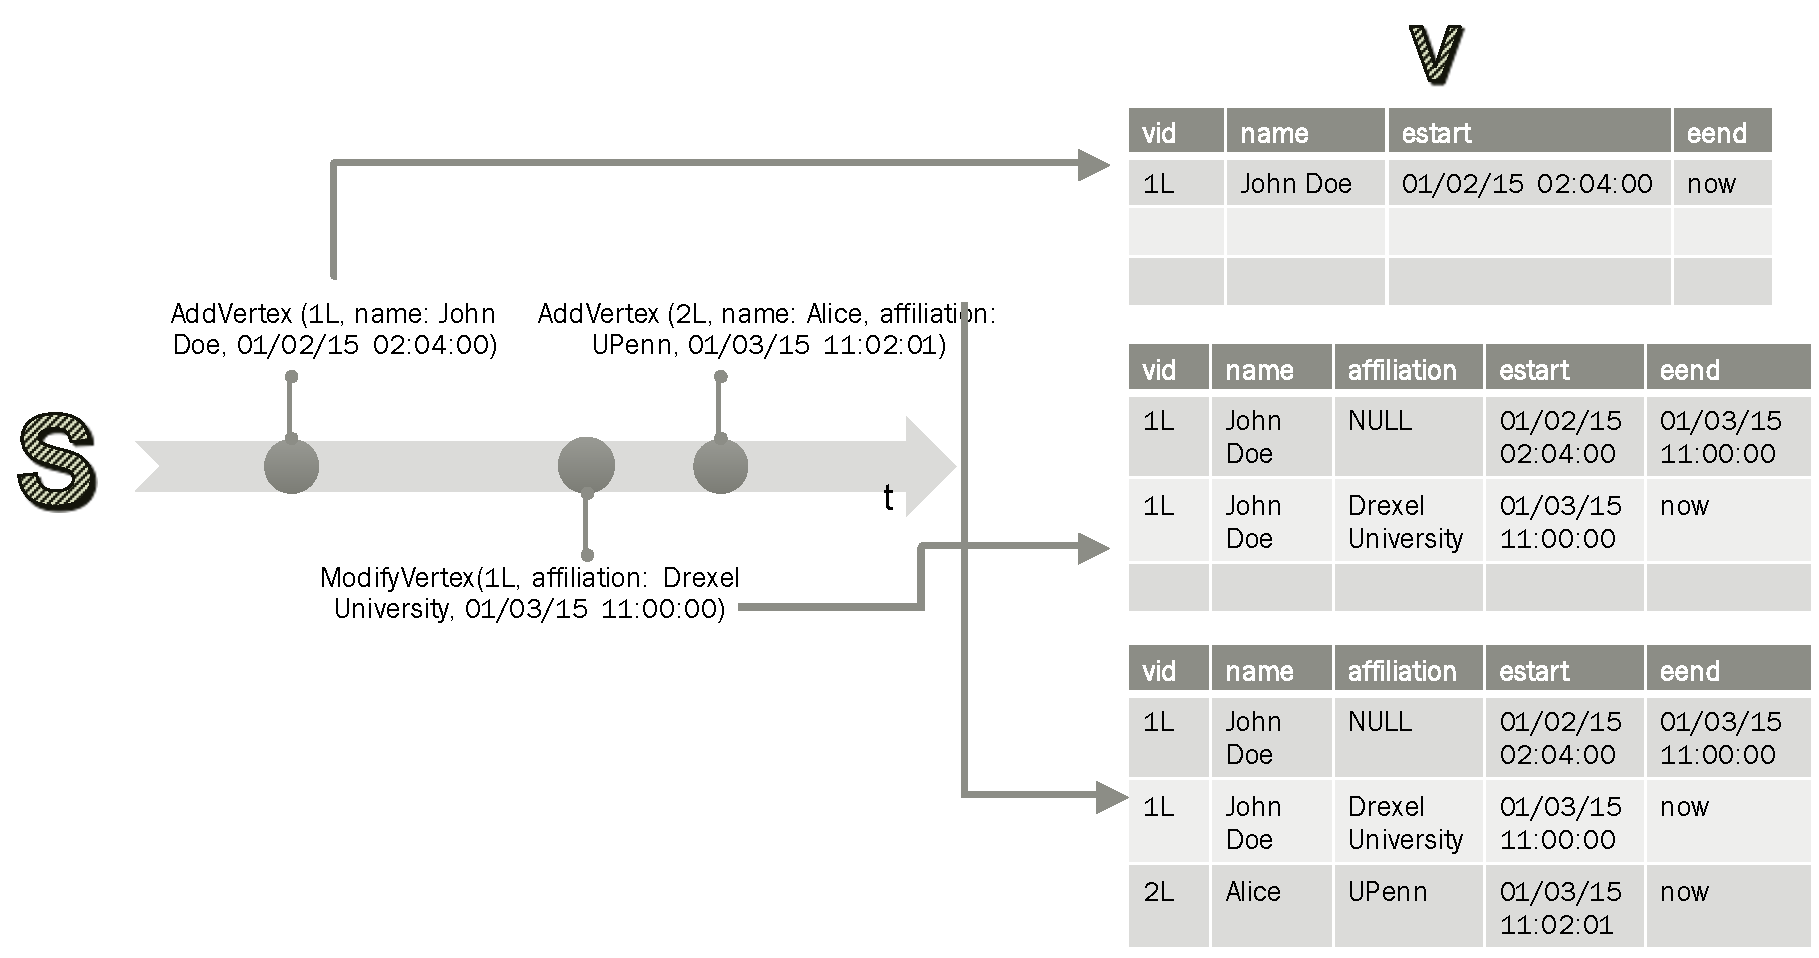
\includegraphics[width=6in]{figs/stream_to_state.pdf}
\caption{Stream $S$ emits graph change events which are converted to
  evolving graph state model $TG$.}
\label{fig:streamtotg}
\end{figure*}

Because the stream emits {\em individual entities} rather than {\em
  whole graphs}, graph snapshots can only be reconstructed by
maintaining the history of changes over time.  Our evolving graph
model can be easily constructed from the change stream model following
the conventional temporal database approach
(Figure~\ref{fig:streamtotg}):
\begin{itemize}[noitemsep,topsep=0pt]
\item For an Add event at time $t_i$, add a new tuple with $p=[t_i,
  now)$
\item For a Delete event at time $t_i$, modify the tuple matching the
  primary key by setting $p=[t_s, now)$ to $[t_s, t_i)$.
\item For a Change event at time $t_i$, modify the tuple matching the
  primary key as for a Delete event, and add a new tuple with the
  changed value as for an Add event.
\end{itemize}

This approach assumes that no events arrive out of order and there are
no redundant or duplicate events.  However, it would be a simple
extension to relax these two assumptions.  We also use a closed world
assumption -- if no event is recorded, for our purposes it did not
occur.

\subsection{Algebra}
\label{sec:model:algebra}

All operations in our model take one or two \tgs and return a \tg,
i.e. the algebra is compositional.  More importantly, all operations
maintain the integrity of the model by computing the value of $V$,
followed by the value of $E$, maintaining the foreign key constraint
from $E$ to $V$ and the maximally coalesced non-overlapping time
period contraint on both $V$ and $E$.

\begin{definition}[Selection]
Temporal and structural selection on $TG$ is a selection on the
attributes of $V$ and $E$.  Subgraph is $\sigma_{a \theta v}(TG)$,
where $a$ are attributes of $V$ and/or $E$, $\theta$ is a binary
operation in the set $\{<, \leq, =, \neq, \geq, >\}$, and $v$ is a
value constant.  Temporal selection over $TG$ is $\sigma_{[a,b)}(TG) =
  \{t: t \in TG, t(p).overlaps(period(a,b))\}$ which returns a subset
  of $TG$ within the bounds of $[a,b)$.
\label{def:selection}
\end{definition}

In SQL, temporal selection can be expressed as follows for $V$
(similarly for $E$):

\begin{small}
\begin{verbatim}
SELECT vid, a1, ..., an, greatest(estart, DATE ':date1'), 
       least(eend, DATE ':date2')
FROM V
WHERE eperiod OVERLAPS PERIOD (DATE ':date1', DATE ':date2')
\end{verbatim}
\end{small}

Temporal and structural selection are supported by the same selection
operator and can be used together.  For example, one could select a
sub-graph in an evolving co-citation network of only authors whose
names start with letter A, over the past decade.  Because of the
constraint on $E$, even if the structural selection is only on
attributes of $V$, only edges connecting selected vertices are
retained.  Neither deduplication nor coalescing is required as a
post-operation.

\begin{definition}[Projection]
Projection on $TG$ is projection on attributes of $V$ and $E$ with
coalescing, i.e. \\$\Pi vid, p, a_1, \ldots, a_n(V); \Pi vid_1, vid_2,
p, b_1, \ldots, b_m(E)$. 
\label{def:projection}
\end{definition}

The primary key is always retained, so deduplication is not necessary.
However, coalescing is always performed.  Projection and coalescing
can be expressed in temporal SQL as follows in a structure-only case:

\begin{small}
\begin{verbatim}
CREATE VIEW ProjV(vid, estart, eend) AS (
  SELECT vid, estart, eend FROM V);
CREATE VIEW ProjE(vid1, vid2, estart, eend) AS (
  SELECT vid1, vid2, estart, eeend FROM E);
CREATE VIEW CoalescV(vid, estart, eend) AS (
  SELECT DISTINCT F.vid, F.estart, L.eend
  FROM ProjV F, ProjV L
  WHERE F.estart < L.eend AND F.vid = L.vid
  AND NOT EXISTS (SELECT * FROM ProjV M
    WHERE M.vid = F.vid
    AND F.estart < M.estart AND M.estart <= L.eend
    AND NOT EXISTS (SELECT * From ProjV M1
      WHERE M1.vid = F.vid
      AND M1.estart < M.estart
      AND V.estart <= M1.eend ) )
  AND NOT EXISTS (SELECT * from ProjV M2
    WHERE M2.vid = F.vid
    AND ( (M2.estart < F.estart AND F.estart <= M2.eend)
    OR (M2.estart <= L.eend AND L.eend < M2.eend) ) ) );
CREATE VIEW CoalescE(vid1, vid2, estart, eend) AS (
  SELECT DISTINCT F.vid1, F.vid2, F.estart, L.eend
  FROM ProjE F, ProjE L
  WHERE F.estart < L.eend AND F.vid1 = L.vid1 
  AND F.vid2 = L.vid2
  AND NOT EXISTS (SELECT * FROM ProjE M
    WHERE M.vid1 = F.vid1 AND M.vid2 = F.vid2
    AND F.estart < M.estart AND M.estart <= L.eend
    AND NOT EXISTS (SELECT * From ProjE M1
      WHERE M1.vid1 = F.vid1
      AND M1.vid2 = F.vid2
      AND M1.estart < M.estart
      AND V.estart <= M1.eend ) )
  AND NOT EXISTS (SELECT * from ProjE M2
    WHERE M2.vid1 = F.vid1 AND M2.vid2 = F.vid2
    AND ( (M2.estart < F.estart AND F.estart <= M2.eend)
    OR (M2.estart <= L.eend AND L.eend < M2.eend) ) ) )
\end{verbatim}
\end{small}

As already mentioned, snapshots represent the state of the graph at a
particular time instant $t$.  It is often useful to instead analyze
the graph as an aggregation over some time period $p$.  We call such a
graph a {\em representative graph}.  For example, a union of all
vertices/edges over 1 month is representative of that graph during
that month.  Analysis of representative graphs can lead to deeper
insight than of a snapshot.  For example, a co-authorship network DBLP
is very sparse - one can only publish so many papers in any given
month - on a daily or even monthly level of granularity, but can show
community formation and affiliation when aggregated over multiples of
years.  From this perspective, an evolving graph is a sequence of
representative graphs over consecutive arbitrary-length periods.

In SQL, the representative graph periods can be computed as follows:

\begin{small}
\begin{verbatim}
CREATE VIEW Changes(day) as (
  SELECT DISTINCT estart FROM V
  UNION SELECT DISTINCT eend FROM V
  UNION SELECT DISTINCT estart from E
  UNION SELECT DISTINCT eend FROM E);
CREATE VIEW ChangePeriods(estart, eend) as (
  SELECT P1.day, P2.day
  FROM Changes P1, Changes P2
  WHERE P1.day < P2.day AND NOT EXISTS (
     SELECT * from Changes P3
     WHERE P1.day < P3.day and P3.day < P2.day ) )
\end{verbatim}
\end{small}

\begin{figure}
\centering
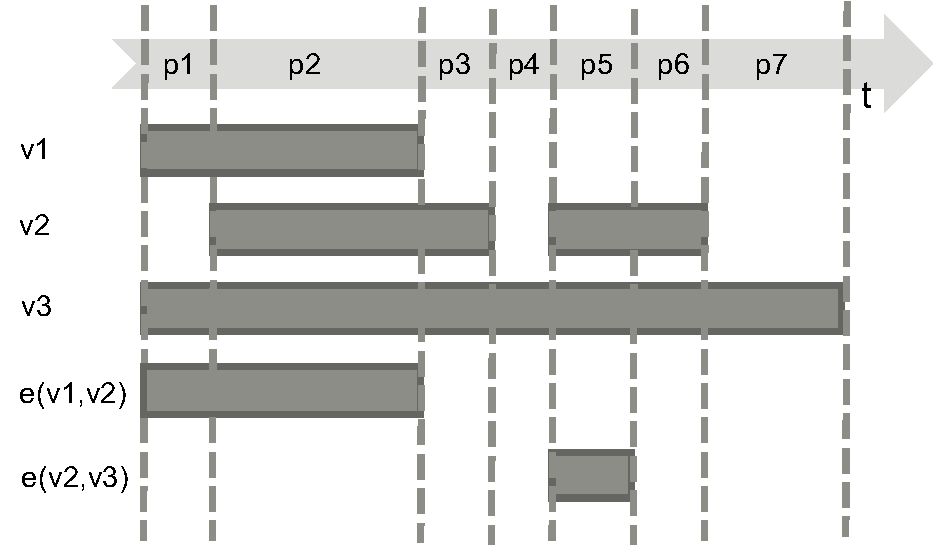
\includegraphics[width=3.4in]{figs/change_timeline.pdf}
\caption{The regions of constant value within the whole graph compose
  representative graphs.}
\label{fig:changes}
\end{figure}

An example in Figure~\ref{fig:changes} illustrates this concept.

Here we propose a general way to aggregate evolving graphs over our
model.  This approach is based on the stream aggregation work by Li,
et al.~\cite{Li2005} with addition of quantifiers.  Aggregation is
performed through specification of time windows.  Windows can be
defined in terms of {\em time} or {\em change}.  The time window is
semantic and can be any multiples of $\{minutes, hours, days, weeks,
\\ months, years\}$, i.e. the usual time units.  The window span
itself is based on absolute values rather than from some starting
point and direction.  Thus, window specification of 1 year would
produce windows for each calendar year occurring in the data.  The
{\em change} type is equivalent to the time period of one
representative graph, i.e. period during which all the graph values
are constant (this is similar to the slide-by-row type in stream
aggregation).

Aggregation in relational algebra produces results for each grouping
irrespective of how many results there are, unless a \insql{HAVING}
restriction is applied.  The quantification over the aggregation
results in evolving graphs is useful for producing different kinds of
representative graphs.  For example, to produce a representative graph
with only strong connections over a volatile evolving graph, we want
to restrict results to those edges that span the entire window or a
large subset of that window.  For this purpose we introduce
quantifiers.

Hsu and Parker define a ``{\em generalized quantifier} $Q(R)$ as a
Boolean-valued function of a relation'' ~\cite{Hsu1995}.  A quantifier
contains an {\em n-place determiner}.

For example, ``at least one vertex in each window for each group'' is
a 2-place determiner quantifier which has the existential semantics.
Many kinds of quantifiers are possible.  In our work we restrict the
determiners to be from the set $\{at\ least\ one, all, most,
at\ least\ n\}$, where $n$ is an integer representing a ratio.  $all$
is a usual universal quantifier that in standard SQL can be achieved
with the use of two \insql{NOT EXISTS}.

Now that we have the window semantics and quantification defined, we
can define the aggregation operation over an evolving graph $TG$.

\begin{definition}[Evolving Graph Aggregation]
An {\em aggregation} operation over $TG$ is a function \\ $G_1, G_2,
\ldots, G_n, W, Q g f_1(A_1), f_2(A_2), \ldots, f_m(A_m)(TG)$, where
each $G_i$ is a grouping attribute from $TG$ with the exception of
$p$; $W$ is the window specification; $Q$ is a generalized quantifier
specification for vertices and edges on the coverage of the window;
each $F_i$ is an aggregation function; and each $A_i$ is an attribute
name from $TG$.
\label{def:agg}
\end{definition}

This definition is similar to the regular relational algebra
aggregation definition, with the addition of the window specification
and the restriction of grouping attributes to exclude the time
periods.  However, both $V$ and $E$ relations are aggregated by the
same operation and the constraint on $E$ to contain only those
vertices that exist in $V$ is maintained.  The aggregation defined
this way allows to aggregate graphs structurally, temporally, or in
combination.  To aggregate only temporally, the grouping attribute
must be $vid$ for $V$ and $(vid1, vid2)$ for $E$.  To aggregate only
structurally, the window specification must be by 1 change.  Observe
that aggregation by 1 change with grouping by id is a no-op, and in
fact the sequence of representative graphs on the source data is equal
to the deduplicated sequence of snapshots.

The quantifier is applied to the coverage of the window period within
each grouping.  For example, to construct the persistent edges graph
from the example above, we use the $all$ quantifier over the $E$ relation.
Only the edges that span the duration of the window period are
produced.  Since the universal quantification is very restrictive,
$most$ and $at\ least\ n$ quantifiers are more appropriate in some
aggregations, especially over long windows.  To obtain a stable
1-month graph over an evolving network connections graph, we may ask
for connections that exist in at least 90\% of the period.

Remember that the schema for $V$ has a $(vid, p)$ primary key.  Any
aggregation operation must produce both a valid $vid$ and valid time
interval for each tuple.  We produce a $vid$ by using the hash of the
grouping variables to maintain temporal consistency.  The time
interval is produced by the window extent from the window
specification. Similarly for $E$.

The aggregation functions over the selected graph attributes are used
to compute the new value representative of the whole window.  We
support the standard set $\{count, min,$ $max, sum, average\}$, as
well as $\{any, first, last, list\}$.  $first$ and $last$ refer to
first/last non-null value in the window and are possible because the
aggregating tuples have the time dimension, and the ties are decided
arbitrarily.  $count$ is the count of the number of distinct values
over the aggregation window.  Additional aggregation functions can be
defined by the user.

\begin{figure*}
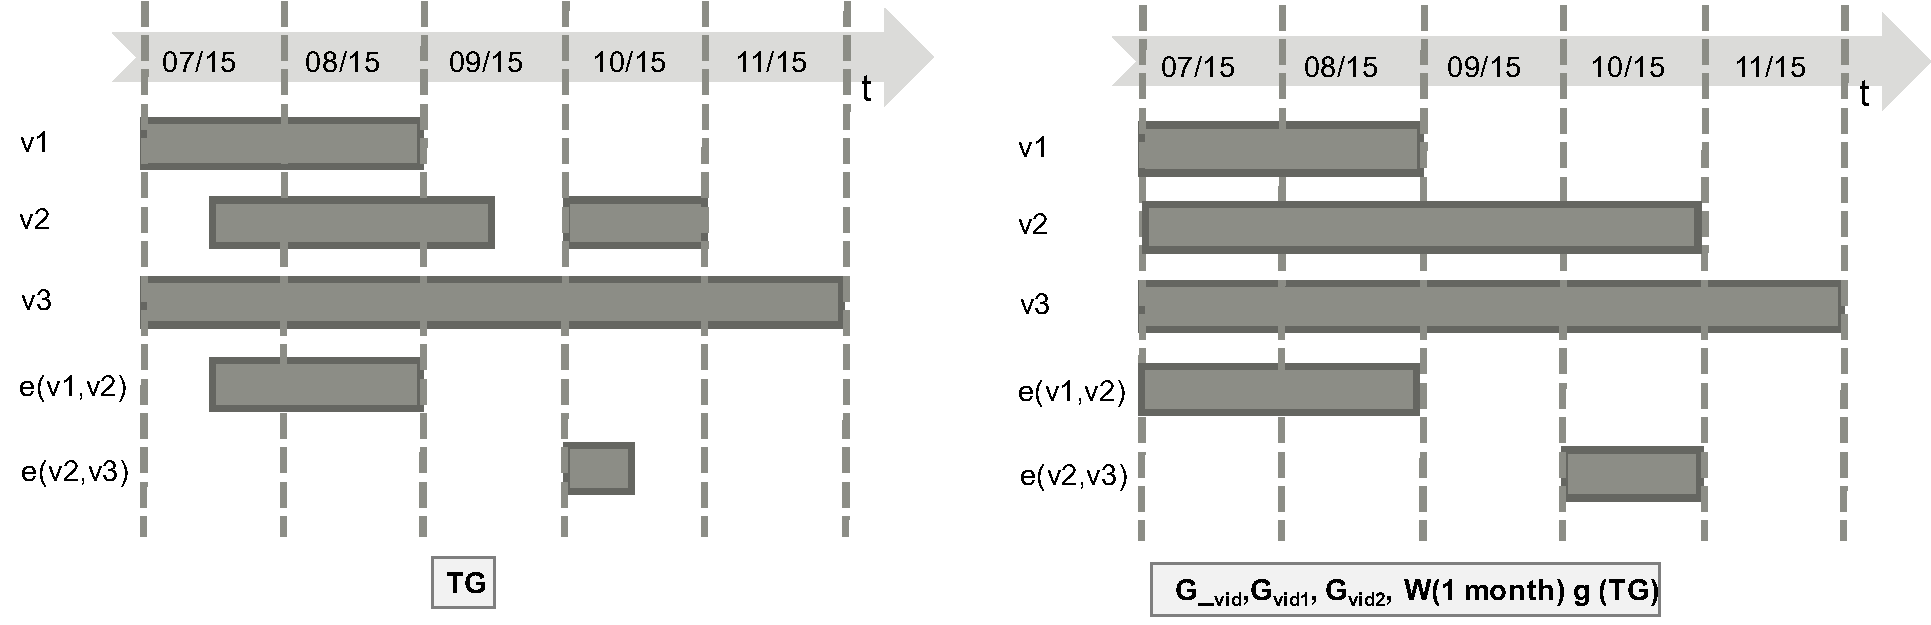
\includegraphics[width=6.5in]{figs/agg1.pdf}
\caption{1-month window aggregation with grouping by id, with
  existential vertex/edge quantifier.  Structure only.}
\label{fig:agg1}
\end{figure*}

An example in Figure~\ref{fig:agg1} shows a small \tg and a result of
aggregation by 1 month on that graph with $at\ least\ one$ quantifier,
with group by id.

It is possible but difficult to express the aggregation operation as
defined above in temporal SQL because each tuple may belong to
multiple windows.

\begin{definition}[Union]
Union of $TG1\ \cup\ TG2$ = $\{v, e: v \in TG1.V$ or $v \in TG2.V$ or
$v(vid$, $f_1(a_{11}$, $a_{21})$, \ldots, $f_n(a_{1n}, a_{2n})$,
$period(least(p_1, p_2), greatest(p_1, p_2)))$, $e \in TG1.E$ or $e
\in TG2.E$ or $e(vid1, vid2, g_1(b_{11}, b_{21}), \ldots, g_m(b_{1m},
b_{2m})$, $period(least(p_1, p_2), greatest(p_1, p_2))) \}$, where
each $f$, respectively $G$, is an aggregation function over one
vertex, respectively edge, attribute where the values intersect over
some period $p$.
\label{def:union}
\end{definition}

\begin{figure*}
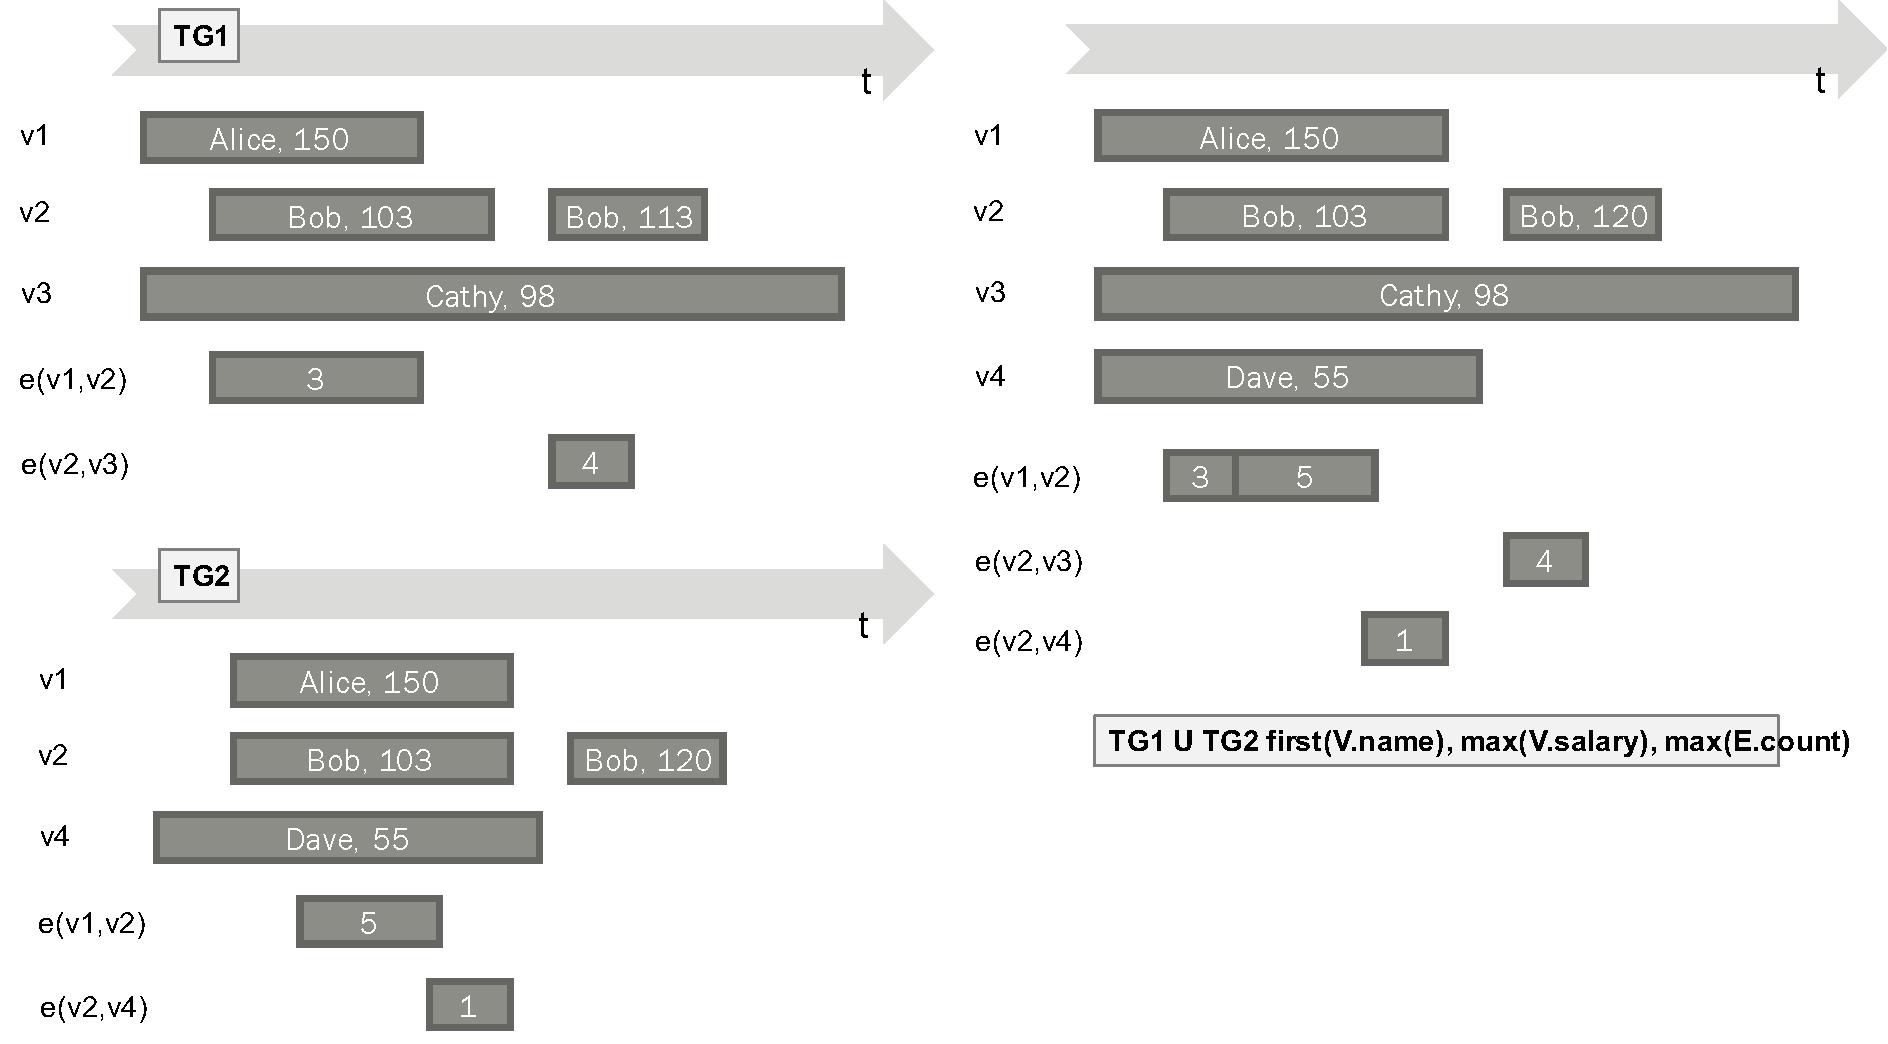
\includegraphics[width=6.5in]{figs/union.pdf}
\caption{Union of TG1 and TG2.}
\label{fig:union}
\end{figure*}

In other words, union of two \tgs is simply all vertices and edges
from both \tgs, with vertex/edge attributes decided by specified
aggregation functions for each period where both values are present,
with coalescing.  Figure~\ref{fig:union} illustrates this concept.

Similarly, intersection of two \tgs is an intersection of
vertices/edges of two graphs, with values for each overlapping
attribute computed by a specified aggregate function.
